%%%%%%%%%%%%%%%%%%%%%%%%%%%%%%%%%%%%%%%%%
% eBook 
% LaTeX Template
% Version 1.0 (29/12/14)
%
% This template has been downloaded from:
% http://www.LaTeXTemplates.com
%
% Original author:
% Luis Cobo (luiscobogutierrez@gmail.com) with extensive modifications by:
% Vel (vel@latextemplates.com)
%
% License:
% CC BY-NC-SA 3.0 (http://creativecommons.org/licenses/by-nc-sa/3.0/)
%
%%%%%%%%%%%%%%%%%%%%%%%%%%%%%%%%%%%%%%%%%

%----------------------------------------------------------------------------------------
%	DOCUMENT CONFIGURATIONS AND INFORMATION
%----------------------------------------------------------------------------------------
 
%%%%%%%%%%%%%%%%%%%%%%%%%%%%%%%%%%%%%%%%%
% eBook
% Structural Definitions File
% Version 1.0 (29/12/14)
%
% Created by:
% Vel (vel@latextemplates.com)
% 
% This file has been downloaded from:
% http://www.LaTeXTemplates.com
%
% License:
% CC BY-NC-SA 3.0 (http://creativecommons.org/licenses/by-nc-sa/3.0/)
%
%%%%%%%%%%%%%%%%%%%%%%%%%%%%%%%%%%%%%%%%%

%----------------------------------------------------------------------------------------
%	REQUIRED PACKAGES
%----------------------------------------------------------------------------------------

\usepackage[portuguese]{babel}

\usepackage[utf8]{inputenc} % Required for inputting international characters
% \usepackage[T1]{fontenc} % Output font encoding for international characters

\usepackage[osf]{libertine} % Use the Libertine font
% \usepackage{microtype} % Improves character and word spacing

\usepackage{tikz} % Required for drawing custom shapes
\definecolor[named]{color01}{rgb}{.2,.4,.6} % Color used in the title page
\usepackage{wallpaper} % Required for setting background images (title page)

\usepackage[unicode=true,bookmarks=true,bookmarksnumbered=false,bookmarksopen=false,breaklinks=false,pdfborder={0 0 1},backref=section,colorlinks=false]{hyperref} % PDF meta-information specification

\usepackage{tikz}
\usepackage{tikzpagenodes}

%----------------------------------------------------------------------------------------
%	PAPER, MARGIN AND HEADER/FOOTER SIZES
%----------------------------------------------------------------------------------------

\setstocksize{22.5cm}{14.1cm} % Paper size
\settrimmedsize{\stockheight}{\stockwidth}{*} % No trims
\setlrmarginsandblock{25pt}{25pt}{*} % Left/right margins
\setulmarginsandblock{30pt}{36pt}{*} % Top/bottom margins
\setheadfoot{14pt}{12pt} % Header/footer height
\setheaderspaces{*}{8pt}{*} % Extra header space
 
%----------------------------------------------------------------------------------------
%	FOOTNOTE CUSTOMIZATION
%----------------------------------------------------------------------------------------

\renewcommand{\foottextfont}{\itshape\footnotesize} % Font settings for footnotes
\setlength{\footmarkwidth}{-.1em} % Space between the footnote number and the text
\setlength{\footmarksep}{.1em} % Space between multiple footnotes on the same page
\renewcommand*{\footnoterule}{} % Remove the rule above the first footnote
\setlength{\skip\footins}{1\onelineskip} % Space between the body text and the footnote

%----------------------------------------------------------------------------------------
%	HEADER AND FOOTER FORMATS
%----------------------------------------------------------------------------------------

\makepagestyle{mio} % Define a new custom page style
\setlength{\headwidth}{\textwidth} % Header the same width as the text
\makeheadrule{mio}{\textwidth}{0.1mm} % Header rule height
\makeoddhead{mio}{\scriptsize{\theauthor\hskip.2cm\vrule\hskip.2cm\itshape{\thetitle}}}{}{} % Header specification
\makeoddfoot{mio}{}{\scriptsize {\thepage \quad \vrule \quad \thelastpage}}{} % Footer specification
\makeoddfoot{plain}{}{\footnotesize {\thepage \quad \vrule \quad \thelastpage}}{} % Pages of chapters
\pagestyle{mio} % Set the page style to the custom style defined above

%----------------------------------------------------------------------------------------
%	PART FORMAT
%----------------------------------------------------------------------------------------

\renewcommand{\partnamefont}{\centering\sffamily\itshape\Huge} % Part name font specification
\renewcommand{\partnumfont}{\sffamily\Huge} % Part number font specification
\renewcommand{\parttitlefont}{\centering\sffamily\scshape} % Part title font specification
\renewcommand{\beforepartskip}{\null\vskip.618\textheight} % Whitespace above the part heading

%----------------------------------------------------------------------------------------
%	CHAPTER FORMAT
%----------------------------------------------------------------------------------------

\makechapterstyle{Tufte}{ % Define a new chapter style
	\renewcommand{\chapterheadstart}{\null \vskip3.5\onelineskip} % Whitespace before the chapter starts
	\renewcommand{\printchaptername}{\large\itshape\chaptername} % "Chapter" text font specification
	\renewcommand{\printchapternum}{\LARGE\thechapter \\} % Chapter number font specification
		\renewcommand{\afterchapternum}{} % Space between the chapter number and text
		\renewcommand{\printchaptertitle}[1]{ % Chapter title font specification
			\raggedright
			\itshape\Huge{##1}}
		\renewcommand{\afterchaptertitle}{
			\vskip3.5\onelineskip
	}}
	\chapterstyle{Tufte} % Set the chapter style to the custom style defined above
				
	%----------------------------------------------------------------------------------------
	%	SECTION FORMAT
	%----------------------------------------------------------------------------------------
				
	\setsecheadstyle{\sethangfrom{\noindent ##1}\raggedright\sffamily\itshape\Large} % Section title font specification
	\setbeforesecskip{-.6\onelineskip} % Whitespace before the section
	\setaftersecskip{.3\onelineskip} % Whitespace after the section
				
	%----------------------------------------------------------------------------------------
	%	SUBSECTION FORMAT
	%----------------------------------------------------------------------------------------
				
	\setsubsecheadstyle{\sethangfrom{\noindent  ##1}\raggedright\sffamily\large\itshape} % Subsection title font specification
	\setbeforesubsecskip{-.5\onelineskip} % Whitespace before the subsection
	\setaftersubsecskip{.2\onelineskip} % Whitespace after the subsection
				
	%----------------------------------------------------------------------------------------
	%	SUBSUBSECTION FORMAT
	%----------------------------------------------------------------------------------------
				
	\setsubsubsecheadstyle{\sethangfrom{\noindent ##1}\raggedright\sffamily\itshape} % Subsubsection title font specification
	\setbeforesubsubsecskip{-.5\onelineskip} % Whitespace before the subsubsection
	\setaftersubsubsecskip{.1\onelineskip} % Whitespace after the subsubsection
				
	%----------------------------------------------------------------------------------------
	%	CAPTION FORMAT
	%----------------------------------------------------------------------------------------
				
	\captiontitlefont{\itshape\footnotesize} % Caption font specification
	\captionnamefont{\footnotesize} % "Caption" text font specification
				
	%----------------------------------------------------------------------------------------
	%	QUOTATION ENVIRONMENT FORMAT
	%----------------------------------------------------------------------------------------
				
	\renewenvironment{quotation}
	{\par\leftskip=1em\vskip.5\onelineskip\em}
	{\par\vskip.5\onelineskip}
				
	%----------------------------------------------------------------------------------------
	%	QUOTE ENVIRONMENT FORMAT
	%----------------------------------------------------------------------------------------
				
	\renewenvironment{quote}
	{\list{}{\em\leftmargin=1em}\item[]}{\endlist\relax}
				
	%----------------------------------------------------------------------------------------
	%	MISCELLANEOUS DOCUMENT SPECIFICATIONS
	%----------------------------------------------------------------------------------------
				
	\setlength{\parindent}{1em} % Paragraph indentation
				
	\midsloppy % Fewer overfull lines - used in the memoir class and allows a setting somewhere between \fussy and \sloppy
				
	\checkandfixthelayout % Tell memoir to implement the above
 % Include the file that specifies the document structure and layout

\title{Arreal} % Book title
\author{Bruno Duarte Corrêa} % Author
\newcommand{\edition}{First Edition} % Book edition
 
%----------------------------------------------------------------------------------------

\begin{document}



%----------------------------------------------------------------------------------------
%	TITLE PAGE
%----------------------------------------------------------------------------------------
 
\thispagestyle{empty} % Suppress page numbering
\ThisCenterWallPaper{1.0}{./images/capa} % Add the background image, the first argument is the scaling - adjust this as necessary so the image fits the entire page

% 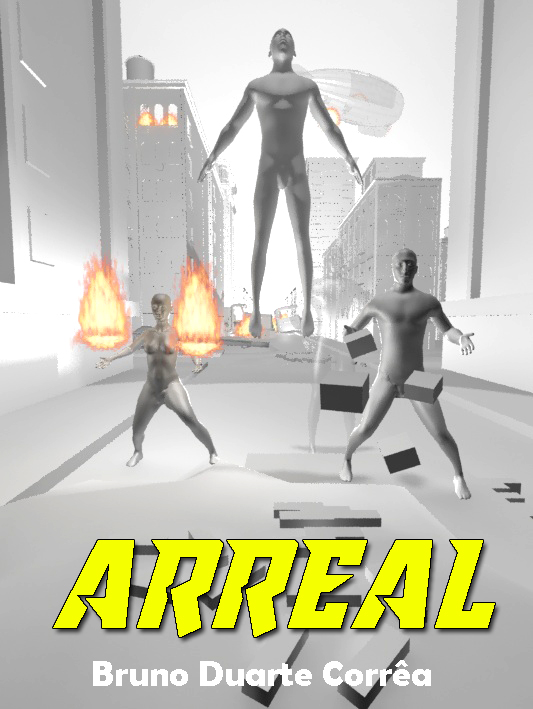
\includegraphics[width=12.5cm]{./images/cover}

% \begin{tikzpicture}[remember picture,overlay]
% \node [rectangle, rounded corners, fill=white, opacity=0, anchor=south west, minimum width=10cm, minimum height=6cm] (box) at (-0.5,-10) (box){}; % White rectangle - "minimum width/height" adjust the width and height of the box; "(-0.5,-10)" adjusts the position on the page
% \node[anchor=west, color01, xshift=-1.5cm, yshift=-5cm, text width=2.9cm, font=\sffamily\bfseries] at (box.north){\theauthor}; % "Text width" adjusts the wrapping width, "xshift/yshift" adjust the position relative to the white rectangle
% \end{tikzpicture}

\newpage\null\thispagestyle{empty}\newpage

\newpage % Make sure the following content is on a new page
 
%----------------------------------------------------------------------------------------
%	TABLE OF CONTENTS
%----------------------------------------------------------------------------------------

% \tableofcontents % Prints the table of contents

% \chapter*{Sinopse}
Já ouvimos muitas histórias sobre superpoderes, heróis, vilões. Muitas foram as vezes em que em uma realidade paralela, fomos salvos por alguém com poderes sobrenaturais, alguém que jamais poderíamos ser iguais, muitas outras tantas também imaginamos como seria poder voar, ou poder ter super. força. A realidade é que não concebemos tal hipótese como ao menos remotamente viável, principalmente à medida que crescemos e de certa forma perdemos a coragem de nos deixar levar para outras realidades ou mesmo questionar o óbvio.
Você já se perguntou como seria se descobrisse que tudo o que acredita ser ilusão ou fantasia, na realidade é a mais pura verdade?
Como lidaria com a possibilidade de poder fazer mais do que sempre fez?
Arreal é uma análise que propõem investigar como reagiríamos em um mundo em que podemos fazer muito mais do que sempre fizemos, bastando acreditar que somos capazes. 
Sabendo que pode realizar algo até então sobrenatural, como voar ou criar realidades paralelas nas mentes de outras pessoas e que ao essas pessoas acreditarem que também são capazes, assim seriam, muitas são as bifurcações de possibilidades.
O que aconteceria caso tal conhecimento de que todos podem fazer coisas extraordinárias caísse nas mãos das pessoas erradas? 
Muitos provavelmente lidariam como algo libertador, mas muitos usariam como poder para escravizar e subjugar.
Saberemos lidar bem com essa realidade?


\foreach \chapternumber in {0,...,44}{
	\input{chapters/chapter\chapternumber.tex}
} 

\chapter*{Nota do Autor}
Essa história sempre foi algo que vivia no fundo da minha mente e sabia que um dia precisava colocar no papel. Desde pequeno para quem me conhecem sabe que nutri a esperança de um dia poder voar com minhas próprias forças, algo como um super herói. Escrever até o final foi pra mim como que um processo terapeutico ao tentar construir personagens que fossem vivos e tivessem seus anseios e depois lendo notei que em cada um deles tinha um pouco de mim. Talvez um pouco do garoto que acha que pode resolver tudo com super poderes mas na verdade não percebe que os grandes problemas da vida na verdade são parte da nossa jornada e que lidar com cada um dos momentos com a força que temos é muito mais forte do que sair voando de uma situação ou ficar invisível pra que ninguém nos veja.

No tempo que levei pra escrever e reler e revissar esse livro, pude refletir sobre o por que eu quero resolver as coisas com poderes e não lidar com elas frente a frente. Hoje em dia me sinto um pouco mais pronto pra lidar com minhas ansiedades e angústias com as armas que tenho.



\begin{tikzpicture}[remember picture, overlay]
    \node[anchor=south west, align=left] at (current page text area.south west) {Apesar de no fundo ainda ter a crença que um dia poderei voar.};
  \end{tikzpicture}
  
  
  
  




\end{document}
